\chapter{Stand der Technik}
\label{chap:technikStand}
%\section{Theorien}
%\section{Techniken}
    Zur Analyse des aktuellen Standes der Technik und Forschung in Bezug zur Konzeption von Software-Lösungen, mit denen 
    die formalisierten Interaktionen der Softwareentwickler vereinfacht werden können, erfolgt in diesem 
    Kapitel ein systematisches Literaturreview. Die Literaturprüfung wird gemäß den Richtlinien, die in der Publikation 
    von \cite{Kitchenham2007} vorgeschlagen werden, durchgeführt. 

    %\section{Methodiken}
    %\label{sec:methodiken}
    %    Im Rahmen dieser Arbeit wurden zur Informationserhebung zuerst ein systematisches Literaturreview durchgeführt und

    \section{Systematisches Literaturreview}
    \label{subsec:systematischesLiteraturReview}
        Die Thematik des systematischen Literaturreviews wurde bereits in den einleitenden Kapiteln erwähnt. 
        Dieser Abschnitt widmet sich ausschließlich der Anwendung der Richtlinien und dem daraus abgeleiteten Stand der Technik 
        abhängig zu dem in der Arbeit behandelten Thema. 

    \subsection{Ziele des Systematischen Literaturreviews}
        Das Ziel dieses systematischen Literaturreviews ist es, die aktuellen Fortschritte von Smart Home Plattformen und 
        Gateways in Richtung der entwicklerseitigen Benutzerfreundlichkeit zu recherchieren. Dabei liegt der Schwerpunkt 
        auf der Usability und der einfachen Handhabung der formalisierten Interaktionen der Softwareentwickler. Es gilt zu 
        analysieren, ob es in diesem Themenbereich bereits Publikationen und Forschungen gibt und welche Entscheidungen 
        getroffen werden müssen, um die Weiterentwicklung eines Systems nicht je nach hinzukommender Funktionalität oder 
        auch Bedingung komplexer werden zu lassen. Die Ergebnisse dieses systematischen Literaturreviews sollen daraufhin 
        als Grundlage der Konzeption einer solchen Plattform dienen und mit einfließen. 

    \subsection{Suchstrategie- und anfragen}
        Dieser Abschnitt beschreibt die Suchstrategie und die Anfragen zu dem systematischen Literaturreview. Hierbei wird 
        erläutert, anhand welcher Kriterien die Literatur ausgewählt wird.
        \\
        In den ersten Schritten werden anhand der Forschungsfragen in Kapitel (\ref{sec:forschungsfragen}) die Stichpunkte 
        aufgegriffen und als Suchterm formuliert. Die daraus resultierenden Suchterme, die der tabellarischen Darstellung 
        (\ref{tab:slr}) zu entnehmen sind, werden in diversen wissenschaftlichen Fachdatenbanken recherchiert und analysiert. 
        Die Ergebnisse werden nach ihrem Titel und der Zusammenfassung sortiert. Gibt es Publikationen mit vergleichbaren 
        Inhalten, so sind diese in weiteren Schritten näher zu betrachten. Damit die Literaturrecherche weitere Ergebnisse 
        erzielt, wird beim studieren der Publikationen die Schneeballsuche angewendet. Dabei wird in den Quellen der jeweiligen 
        Literatur auf weitere Verweise geschaut, die ebenso potentielle Inhalte bearbeiten. Die Kombination beider 
        Literaturergebnisse bilden die Grundlage der zu analysierenden Quellen und geben so den Stand der Technik wieder.
        \begin{figure}[hbt!]
            \centering
            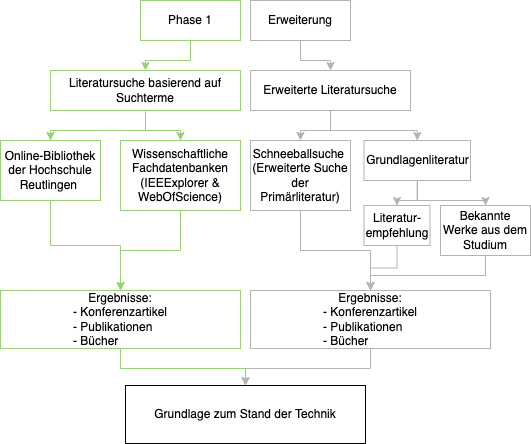
\includegraphics[width=13cm,height=13cm,keepaspectratio]{images/slr_walkthrough.png}
            \caption{Strategie der Literatursuche}
            \label{fig:slr}
        \end{figure}
        \\
        Die generierten Suchterme, die daraus resultierenden Literaturergebnisse und der damit einhergehende Suchverlauf ist 
        zur Nachvollziehbarkeit tabellarisch aufgeführt: 
        \begin{table}[hbt!]
            \begin{center}
                \begin{tabular}{| p{2.8cm} | p{1.9cm} | p{1.7cm} | p{1.9cm} | p{1.9cm} | p{1.8cm} | p{1.8cm} | }
                    \hline
                        \textbf{Suchanfrage} & \textbf{Datum} & \textbf{Filter} & \textbf{Plattform} & \textbf{Ergebnisse} & \textbf{Gesehene} & \textbf{Relevant} \\
                    % \hline
                        % formalized interactions software development & 08.04.2022, 03.05.2022 & Nein & IEEExplorer, WebOfScience & 55, 106 & 5, 4 & 0, 0 \\ 
                    \hline
                        formalized interactions software development architecture  & 11.04.2022, 03.05.2022 & Nein & IEEExplorer, WebOfScience & 13, 26 & 6, 4 & 0, 0 \\ 
                    \hline
                        usability AND formalized interactions AND architecture & 11.04.2022, 03.05.2022 & Nein & IEEExplorer, WebOfScience & 3, 7 & 1, 3 & 0, 1 \\ % A Conceptual Model of Service Customization and Its Implementation
                    \hline
                        usability AND formalized interactions AND architecture AND smart home & 01.05.2022 & Nein & IEEExplorer, WebOfScience & 0, 0 & 0, 0 & 0, 0 \\
                    \hline
                        usability AND formalized interactions AND software development AND architecture & 02.05.2022 & Nein & IEEExplorer, WebOfScience & 1, 1 & 1, 1 & 0, 1 \\
                    \hline
                    %    usability AND formalized interactions AND software development AND architecture AND smart home & 02.05.2022, 03.05.2022 & Nein & IEEExplorer, WebOfScience & 0, 0 & 0, 0 & 0, 0 \\
                    %\hline
                        usability AND architecture AND gateway AND smart home & 06.05.2022 & Nein & IEEExplorer, WebOfScience & 2, 4 & 1, 1 & 1, 1 \\
                    \hline
                        usability AND formalized interaction AND (architecture OR smart home OR software developer OR gateway) & 09.05.2022 & Nein & IEEExplorer, WebOfScience & 3, 10 & 1, 2 & 0, 0 \\
                    \hline
                        usability AND architecture AND smart home AND (formalized interaction OR software developer OR gateway OR iot) & 09.05.2022 & Nein & IEEExplorer, WebOfScience & 13, 22 & 3, 3 & 0, 0 \\
                \end{tabular}
            \end{center}
            \caption{Suchprotokoll des Systematischen Literaturreviews}
            \label{tab:slr}
        \end{table}
        \\
        \pagebreak
    \subsection{Datenextraktion und Synthese}
        Zu der zielgerichteten Datenextraktion werden in Anlehnung an die Richtlinien des systematischen Literaturreviews die folgenden 
        Einschluss- und Ausschlusskriterien definiert, die dabei helfen, die relevanten Publikationen zu finden:
        \begin{table}[hbt!]
            \centering
            \begin{tabular}{p{0.125cm} p{15cm}}
                    \textbf{\#} & \textbf{Einschluss-Kriterien}\\ 
                \hline
                    1  & Die Literatur ist in den wissenschaftlichen Fachdatenbanken veröffentlicht, darunter: WebOfScience, IEEExplorer, SpringerLink, Elsevier, Addison-Wesley, dpunkt-Verlag, ACM und Google Scholar  \\ 
                \hline
                    2  & Der Beitrag wurde nach 2000 veröffentlicht \\ 
                \hline
                    3  & Die Veröffentlichung ist in deutscher oder englischer Sprache \\
                \hline
                    \textbf{\#} & \textbf{Ausschluss-Kriterien}\\ 
                \hline
                    1  & Die Veröffentlichung beinhaltet, bzw. behandelt nicht die Schlagworte usability oder architecture oder formalized interaction  \\ 
                \hline
                    2  & Die Publikation gehört zu der Literatur der Grauzone \\ 
                \hline
                    3  & Die Veröffentlichung hat weniger als 5 Zitationen \\
                \hline
                    4  & Die Literatur hat weniger als 5 Seiten Inhalt \\
            \end{tabular}
            \caption{Einschluss- und Ausschlusskriterien des systematischen Literaturreviews}
            \label{tab:slr_criteria}
        \end{table}
        Mit den Forschungsfragen, den Suchtermen und den Einschluss- und Ausschlusskriterien zu der Quellenrecherche werden die dabei erzielten Ergebnisse 
        studiert und anhand ihres Inhaltes synthetisiert. 
    %\subsection{Analyse und Ergebnisse}
    %\subsection{Zusammenfassung}

    \subsection{Ergebnisse}


    % Ergebniserläuterung, dass speziell zu dem Themenbereich keine explizite Literatur existiert. Alle Ergebnisse decken einen Teilbereich ab und geben Impulse 
    % bei der Entwicklung des Konzepts und weiteres. 
